
\chapter{Variables aléatoires discrètes et loi binomiale}
\competences{définir une loi, calculer et interpréter une espérance, reconnaître et utiliser une loi binomiale}
\section{Cours de référence}
Une variable aléatoire discrète $X$ associe un nombre réel à chaque issue. Sa loi donne les valeurs $x_i$ et les probabilités $p_i=P(X=x_i)$, avec $p_i\geq0$ et $\sum p_i=1$.

\begin{retenir}
L'espérance est $E(X)=\sum_i x_ip_i$. Elle représente la valeur moyenne à long terme lorsque l'expérience est répétée dans les mêmes conditions ; elle n'est pas nécessairement une valeur effectivement prise par $X$.
\end{retenir}

\begin{center}
\begin{tikzpicture}[node distance=9mm and 16mm,every node/.style={draw,circle,inner sep=1.5pt,font=\small}]
\node (a) {1};
\node[below left=of a] (b) {1}; \node[below right=of a] (c) {1};
\node[below left=of b] (d) {1}; \node[below=of a] (e) {2}; \node[below right=of c] (f) {1};
\node[below left=of d] (g) {1}; \node[below left=of e] (h) {3}; \node[below right=of e] (i) {3}; \node[below right=of f] (j) {1};
\draw (a)--(b) (a)--(c) (b)--(d) (b)--(e) (c)--(e) (c)--(f) (d)--(g) (d)--(h) (e)--(h) (e)--(i) (f)--(i) (f)--(j);
\end{tikzpicture}
\end{center}

\begin{retenir}
$X$ suit une loi binomiale $\mathcal B(n,p)$ lorsque $X$ compte le nombre de succès dans $n$ épreuves de Bernoulli indépendantes, de même probabilité de succès $p$. Alors
\[
P(X=k)=\binom nk p^k(1-p)^{n-k},\qquad E(X)=np.
\]
\end{retenir}

Le coefficient $\binom nk$ compte le nombre de chemins contenant exactement $k$ succès parmi $n$ épreuves. Pour $n\leq10$, il peut être lu dans le triangle de Pascal.

\begin{center}
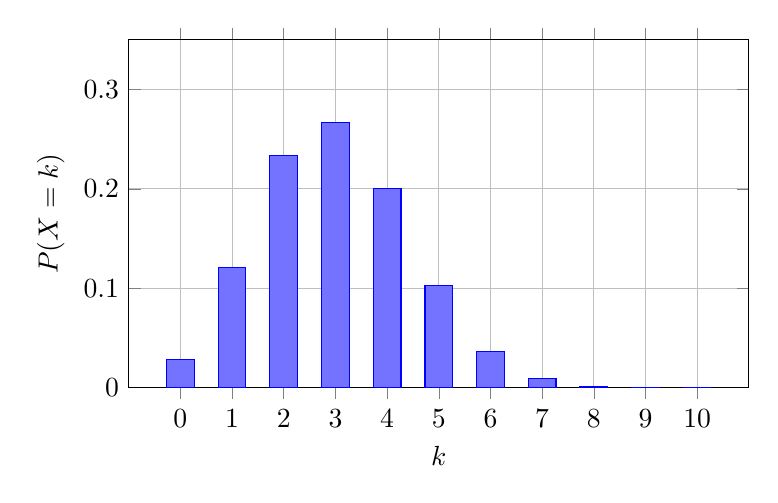
\begin{tikzpicture}
\begin{axis}[ybar,width=.78\textwidth,height=6cm,xlabel={$k$},ylabel={$P(X=k)$},ymin=0,ymax=.35,xtick=data,grid=major]
\addplot[fill=Blue!55,draw=Blue] coordinates {(0,.0282)(1,.1211)(2,.2335)(3,.2668)(4,.2001)(5,.1029)(6,.0368)(7,.0090)(8,.0015)(9,.0002)(10,.0000)};
\end{axis}
\end{tikzpicture}
\end{center}
Le diagramme représente approximativement $\mathcal B(10,0{,}3)$ ; son centre est proche de $E(X)=3$.

\sessionheader{47}{06/04/2027}{B : 2 h -- C : 1 h}{Espérance d'une variable aléatoire}{Variables aléatoires discrètes}
\begin{objectifs}\begin{itemize}\item Définir une loi.\item Calculer une espérance.\item Interpréter une moyenne théorique.\end{itemize}\end{objectifs}
\begin{automatismes}\begin{enumerate}\item Réduire $3x+8-x+2$. \rep{$2x+10$}\item Donner $E(X)$ pour $X\sim\mathcal B(10,0{,}3)$. \rep{$3$}\item Calculer $\binom52$. \rep{$10$}\item Calculer l'espérance de $X$ constant égal à $8$. \rep{$8$}\item Traduire $X\geq1$ par un complémentaire. \rep{$1-P(X=0)$}\end{enumerate}\end{automatismes}
\begin{prerequis}Relire la dernière trace écrite et savoir effectuer les calculs élémentaires mobilisés aujourd'hui. Avant l'activité, faire reformuler les mots-clés : définir une loi et calculer une espérance.\end{prerequis}

\begin{activite}
Un jeu coûte $2$ euros. Le gain brut vaut $0$, $3$ ou $10$ euros avec probabilités $0{,}6$, $0{,}3$, $0{,}1$. Construire la loi du gain net $X$, calculer $E(X)$ et décider si le jeu est favorable au joueur.

\end{activite}
\enseignant{$X$ vaut $-2,1,8$. $E(X)=-1{,}2+0{,}3+0{,}8=-0{,}1$ euro : jeu défavorable en moyenne. Faire verbaliser la donnée qui déclenche le choix de méthode.}

\begin{traceecrite}La loi de $X$ associe à chaque valeur $x_i$ la probabilité $p_i$. L'espérance $E(X)=\sum x_ip_i$ est une moyenne théorique à long terme.\end{traceecrite}

\begin{exemple}
Reprendre les données de l'activité et rédiger la solution dans l'ordre : définition des objets, propriété utilisée, calcul exact ou approché, puis phrase de réponse. La réponse modèle figure dans l'édition enseignant.
\end{exemple}
\enseignant{$X$ vaut $-2,1,8$. $E(X)=-1{,}2+0{,}3+0{,}8=-0{,}1$ euro : jeu défavorable en moyenne.}

\begin{exercice}[-- essentiel]
\begin{enumerate}\item Justifier que le nombre de succès parmi $8$ essais indépendants, avec $p=0{,}3$, suit une loi binomiale.\item Calculer $P(X=2)$ et $P(X=0)$.\item En déduire $P(X\geq1)$ et calculer $E(X)$.\end{enumerate}
\end{exercice}
\enseignant{$X\sim\mathcal B(8,0{,}3)$. $P(X=2)=\binom{8}2 0{,}3^2 0{,}7^{6}$, $P(X=0)=0{,}7^{8}$, $P(X\geq1)=1-P(X=0)$ et $E(X)=\dfrac{24}{10}$.}

\manuelref{Calao, cours p. 154--159 ; exercices p. 160, n° 1 à 5}
\ExoSession{47}

\begin{dm}Reprendre l'exercice d'entraînement 2 avec les données suivantes : remplacer la donnée initiale par $355$ et le taux ou la raison par $7$. Rédiger en quatre lignes : données, formule, calcul, conclusion.\end{dm}
\enseignant{La correction dépend de l'exercice repris. Vérifier surtout la cohérence du modèle, le nombre d'itérations, l'arrondi et la phrase de conclusion.}

\begin{sortie}Sur une demi-feuille : écrire la règle principale de la séance, traiter un exemple très court et indiquer son degré de confiance de 1 à 4. Question(s) essentielle(s) du jour : 1, 2 et 3.\end{sortie}

\ifprof
\begin{methode}
\textbf{Conduite en 1 h :} 7 min d'automatismes ; 10 min de mise en commun et trace ; 28 min d'exercices essentiels ; 5 min de correction ; 3 min de billet de sortie.\\
\textbf{Conduite en 2 h :} ajouter 20 min de recherche de l'activité, 20 min d'institutionnalisation, un second exercice autonome et 10 min de correction comparée.\\
\textbf{Différenciation :} fournir aux élèves fragiles une fiche à quatre cases (données, modèle, calcul, conclusion). Demander aux élèves rapides de produire un contre-exemple, une justification ou une seconde méthode.
\end{methode}
\fi
\sessionheader{48}{08/04/2027}{B : 1 h -- C : 2 h}{Loi binomiale : reconnaître une situation}{Variables aléatoires discrètes}
\begin{objectifs}\begin{itemize}\item Reconnaître un schéma de Bernoulli.\item Identifier $n$ et $p$.\item Définir $X$.\end{itemize}\end{objectifs}
\begin{automatismes}\begin{enumerate}\item Calculer $5\,\%$ de $180$. \rep{$9$}\item Calculer $\binom52$. \rep{$10$}\item Calculer l'espérance de $X$ constant égal à $9$. \rep{$9$}\item Traduire $X\geq1$ par un complémentaire. \rep{$1-P(X=0)$}\item Donner $E(X)$ pour $X\sim\mathcal B(10,0{,}3)$. \rep{$3$}\end{enumerate}\end{automatismes}
\begin{prerequis}Relire la dernière trace écrite et savoir effectuer les calculs élémentaires mobilisés aujourd'hui. Avant l'activité, faire reformuler les mots-clés : reconnaître un schéma de bernoulli et identifier $n$ et $p$.\end{prerequis}

\begin{activite}
Un client accepte une offre avec probabilité $0{,}25$. Un conseiller contacte indépendamment huit clients. Définir $X$, justifier la loi binomiale et identifier $n$ et $p$.

\end{activite}
\enseignant{$X$ compte les acceptations ; répétition de 8 épreuves identiques et indépendantes, succès de probabilité $0{,}25$ : $X\sim\mathcal B(8,0{,}25)$. Faire verbaliser la donnée qui déclenche le choix de méthode.}

\begin{traceecrite}$X\sim\mathcal B(n,p)$ si $X$ compte les succès dans $n$ épreuves indépendantes de même probabilité $p$.\end{traceecrite}

\begin{exemple}
Reprendre les données de l'activité et rédiger la solution dans l'ordre : définition des objets, propriété utilisée, calcul exact ou approché, puis phrase de réponse. La réponse modèle figure dans l'édition enseignant.
\end{exemple}
\enseignant{$X$ compte les acceptations ; répétition de 8 épreuves identiques et indépendantes, succès de probabilité $0{,}25$ : $X\sim\mathcal B(8,0{,}25)$.}

\begin{exercice}[-- essentiel]
\begin{enumerate}\item Justifier que le nombre de succès parmi $9$ essais indépendants, avec $p=0{,}3$, suit une loi binomiale.\item Calculer $P(X=2)$ et $P(X=0)$.\item En déduire $P(X\geq1)$ et calculer $E(X)$.\end{enumerate}
\end{exercice}
\enseignant{$X\sim\mathcal B(9,0{,}3)$. $P(X=2)=\binom{9}2 0{,}3^2 0{,}7^{7}$, $P(X=0)=0{,}7^{9}$, $P(X\geq1)=1-P(X=0)$ et $E(X)=\dfrac{27}{10}$.}

\manuelref{Calao, cours p. 154--159 ; exercices p. 160, n° 5, puis p. 162, n° 14 à 20}
\ExoSession{48}

\begin{dm}Reprendre l'exercice d'entraînement 3 avec les données suivantes : remplacer la donnée initiale par $360$ et le taux ou la raison par $2$. Rédiger en quatre lignes : données, formule, calcul, conclusion.\end{dm}
\enseignant{La correction dépend de l'exercice repris. Vérifier surtout la cohérence du modèle, le nombre d'itérations, l'arrondi et la phrase de conclusion.}

\begin{sortie}Sur une demi-feuille : écrire la règle principale de la séance, traiter un exemple très court et indiquer son degré de confiance de 1 à 4. Question(s) essentielle(s) du jour : 1 et 2.\end{sortie}

\ifprof
\begin{methode}
\textbf{Conduite en 1 h :} 7 min d'automatismes ; 10 min de mise en commun et trace ; 28 min d'exercices essentiels ; 5 min de correction ; 3 min de billet de sortie.\\
\textbf{Conduite en 2 h :} ajouter 20 min de recherche de l'activité, 20 min d'institutionnalisation, un second exercice autonome et 10 min de correction comparée.\\
\textbf{Différenciation :} fournir aux élèves fragiles une fiche à quatre cases (données, modèle, calcul, conclusion). Demander aux élèves rapides de produire un contre-exemple, une justification ou une seconde méthode.
\end{methode}
\fi
\sessionheader{49}{27/04/2027}{B : 2 h -- C : 1 h}{Triangle de Pascal et coefficients binomiaux}{Variables aléatoires discrètes}
\begin{objectifs}\begin{itemize}\item Construire le triangle de Pascal.\item Lire $\binom nk$.\item Interpréter un coefficient.\end{itemize}\end{objectifs}
\begin{automatismes}\begin{enumerate}\item Écrire le coefficient multiplicateur d'une hausse de $10\,\%$. \rep{$1+\dfrac{10}{100}=1{,}10$}\item Calculer l'espérance de $X$ constant égal à $3$. \rep{$3$}\item Traduire $X\geq1$ par un complémentaire. \rep{$1-P(X=0)$}\item Donner $E(X)$ pour $X\sim\mathcal B(10,0{,}3)$. \rep{$3$}\item Calculer $\binom52$. \rep{$10$}\end{enumerate}\end{automatismes}
\begin{prerequis}Relire la dernière trace écrite et savoir effectuer les calculs élémentaires mobilisés aujourd'hui. Avant l'activité, faire reformuler les mots-clés : construire le triangle de pascal et lire $\binom nk$.\end{prerequis}

\begin{activite}
Construire les lignes $n=0$ à $n=6$ du triangle de Pascal. Expliquer le calcul du nombre $15$ de la ligne $6$, puis lire $\binom62$ et $\binom64$.
\begin{center}\begin{tabular}{*{9}{c}}&&&&1&&&&\\&&&1&&1&&&\\&&1&&2&&1&&\\&1&&3&&3&&1&\\1&&4&&6&&4&&1\end{tabular}\end{center}
\end{activite}
\enseignant{Chaque nombre intérieur est la somme des deux nombres situés au-dessus. $\binom62=\binom64=15$. Faire verbaliser la donnée qui déclenche le choix de méthode.}

\begin{traceecrite}Le triangle de Pascal vérifie $\binom nk=\binom{n-1}{k-1}+\binom{n-1}{k}$. Les bords valent $1$.\end{traceecrite}

\begin{exemple}
Reprendre les données de l'activité et rédiger la solution dans l'ordre : définition des objets, propriété utilisée, calcul exact ou approché, puis phrase de réponse. La réponse modèle figure dans l'édition enseignant.
\end{exemple}
\enseignant{Chaque nombre intérieur est la somme des deux nombres situés au-dessus. $\binom62=\binom64=15$.}

\begin{exercice}[-- essentiel]
\begin{enumerate}\item Justifier que le nombre de succès parmi $10$ essais indépendants, avec $p=0{,}3$, suit une loi binomiale.\item Calculer $P(X=2)$ et $P(X=0)$.\item En déduire $P(X\geq1)$ et calculer $E(X)$.\end{enumerate}
\end{exercice}
\enseignant{$X\sim\mathcal B(10,0{,}3)$. $P(X=2)=\binom{10}2 0{,}3^2 0{,}7^{8}$, $P(X=0)=0{,}7^{10}$, $P(X\geq1)=1-P(X=0)$ et $E(X)=\dfrac{30}{10}$.}

\manuelref{Calao, p. 164, n° 24 à 29, puis p. 166, n° 36}
\ExoSession{49}

\begin{dm}Reprendre l'exercice d'entraînement 2 avec les données suivantes : remplacer la donnée initiale par $365$ et le taux ou la raison par $3$. Rédiger en quatre lignes : données, formule, calcul, conclusion.\end{dm}
\enseignant{La correction dépend de l'exercice repris. Vérifier surtout la cohérence du modèle, le nombre d'itérations, l'arrondi et la phrase de conclusion.}

\begin{sortie}Sur une demi-feuille : écrire la règle principale de la séance, traiter un exemple très court et indiquer son degré de confiance de 1 à 4. Question(s) essentielle(s) du jour : 1, 2 et 3.\end{sortie}

\ifprof
\begin{methode}
\textbf{Conduite en 1 h :} 7 min d'automatismes ; 10 min de mise en commun et trace ; 28 min d'exercices essentiels ; 5 min de correction ; 3 min de billet de sortie.\\
\textbf{Conduite en 2 h :} ajouter 20 min de recherche de l'activité, 20 min d'institutionnalisation, un second exercice autonome et 10 min de correction comparée.\\
\textbf{Différenciation :} fournir aux élèves fragiles une fiche à quatre cases (données, modèle, calcul, conclusion). Demander aux élèves rapides de produire un contre-exemple, une justification ou une seconde méthode.
\end{methode}
\fi
\sessionheader{50}{29/04/2027}{B : 1 h -- C : 2 h}{Probabilités binomiales}{Variables aléatoires discrètes}
\begin{objectifs}\begin{itemize}\item Calculer $P(X=k)$.\item Traduire au moins/au plus.\item Utiliser le complémentaire.\end{itemize}\end{objectifs}
\begin{automatismes}\begin{enumerate}\item Réduire $3x+4-x+2$. \rep{$2x+6$}\item Traduire $X\geq1$ par un complémentaire. \rep{$1-P(X=0)$}\item Donner $E(X)$ pour $X\sim\mathcal B(10,0{,}3)$. \rep{$3$}\item Calculer $\binom52$. \rep{$10$}\item Calculer l'espérance de $X$ constant égal à $4$. \rep{$4$}\end{enumerate}\end{automatismes}
\begin{prerequis}Relire la dernière trace écrite et savoir effectuer les calculs élémentaires mobilisés aujourd'hui. Avant l'activité, faire reformuler les mots-clés : calculer $p(x=k)$ et traduire au moins/au plus.\end{prerequis}

\begin{activite}
Pour $X\sim\mathcal B(8,0{,}25)$, calculer $P(X=2)$, $P(X=0)$ puis $P(X\geq1)$. Traduire chaque événement en phrase.
\begin{center}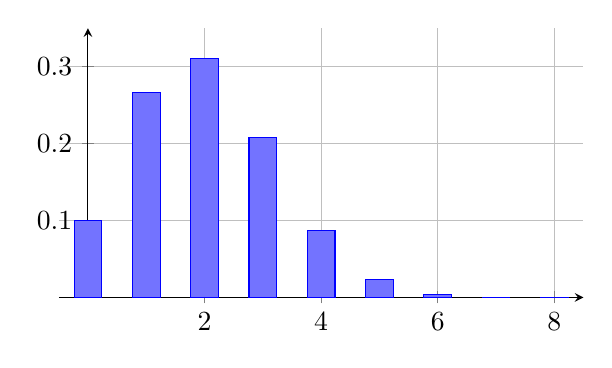
\begin{tikzpicture}\begin{axis}[width=.68\textwidth,height=5cm,axis lines=middle,xmin=-.5,xmax=8.5,ymin=0,ymax=.35,grid=major]\addplot[ybar,fill=Blue!55,draw=Blue] coordinates {(0,.10)(1,.267)(2,.311)(3,.208)(4,.087)(5,.023)(6,.004)(7,.0004)(8,.00002)};\end{axis}\end{tikzpicture}\end{center}
\end{activite}
\enseignant{$P(X=2)=\binom82 0{,}25^2 0{,}75^6\approx0{,}3115$ ; $P(X=0)=0{,}75^8\approx0{,}1001$ ; $P(X\geq1)\approx0{,}8999$. Faire verbaliser la donnée qui déclenche le choix de méthode.}

\begin{traceecrite}Si $X\sim\mathcal B(n,p)$, alors $P(X=k)=\binom nkp^k(1-p)^{n-k}$. Traduire soigneusement « au moins », « au plus » et « aucun ».\end{traceecrite}

\begin{exemple}
Reprendre les données de l'activité et rédiger la solution dans l'ordre : définition des objets, propriété utilisée, calcul exact ou approché, puis phrase de réponse. La réponse modèle figure dans l'édition enseignant.
\end{exemple}
\enseignant{$P(X=2)=\binom82 0{,}25^2 0{,}75^6\approx0{,}3115$ ; $P(X=0)=0{,}75^8\approx0{,}1001$ ; $P(X\geq1)\approx0{,}8999$.}

\begin{exercice}[-- essentiel]
\begin{enumerate}\item Justifier que le nombre de succès parmi $6$ essais indépendants, avec $p=0{,}3$, suit une loi binomiale.\item Calculer $P(X=2)$ et $P(X=0)$.\item En déduire $P(X\geq1)$ et calculer $E(X)$.\end{enumerate}
\end{exercice}
\enseignant{$X\sim\mathcal B(6,0{,}3)$. $P(X=2)=\binom{6}2 0{,}3^2 0{,}7^{4}$, $P(X=0)=0{,}7^{6}$, $P(X\geq1)=1-P(X=0)$ et $E(X)=\dfrac{18}{10}$.}

\manuelref{Calao, p. 164, n° 24 à 29, puis p. 168, n° 41 à 45}
\ExoSession{50}

\begin{dm}Reprendre l'exercice d'entraînement 3 avec les données suivantes : remplacer la donnée initiale par $370$ et le taux ou la raison par $4$. Rédiger en quatre lignes : données, formule, calcul, conclusion.\end{dm}
\enseignant{La correction dépend de l'exercice repris. Vérifier surtout la cohérence du modèle, le nombre d'itérations, l'arrondi et la phrase de conclusion.}

\begin{sortie}Sur une demi-feuille : écrire la règle principale de la séance, traiter un exemple très court et indiquer son degré de confiance de 1 à 4. Question(s) essentielle(s) du jour : 1 et 2.\end{sortie}

\ifprof
\begin{methode}
\textbf{Conduite en 1 h :} 7 min d'automatismes ; 10 min de mise en commun et trace ; 28 min d'exercices essentiels ; 5 min de correction ; 3 min de billet de sortie.\\
\textbf{Conduite en 2 h :} ajouter 20 min de recherche de l'activité, 20 min d'institutionnalisation, un second exercice autonome et 10 min de correction comparée.\\
\textbf{Différenciation :} fournir aux élèves fragiles une fiche à quatre cases (données, modèle, calcul, conclusion). Demander aux élèves rapides de produire un contre-exemple, une justification ou une seconde méthode.
\end{methode}
\fi
\sessionheader{51}{04/05/2027}{B : 2 h -- C : 1 h}{Bilan du chapitre et évaluation}{Variables aléatoires discrètes}
\begin{objectifs}\begin{itemize}\item Calculer et interpréter $E(X)$.\item Résoudre un problème binomial.\item Analyser ses erreurs.\end{itemize}\end{objectifs}
\begin{automatismes}\begin{enumerate}\item Calculer $20\,\%$ de $100$. \rep{$20$}\item Donner $E(X)$ pour $X\sim\mathcal B(10,0{,}3)$. \rep{$3$}\item Calculer $\binom52$. \rep{$10$}\item Calculer l'espérance de $X$ constant égal à $5$. \rep{$5$}\item Traduire $X\geq1$ par un complémentaire. \rep{$1-P(X=0)$}\end{enumerate}\end{automatismes}
\begin{prerequis}Relire la dernière trace écrite et savoir effectuer les calculs élémentaires mobilisés aujourd'hui. Avant l'activité, faire reformuler les mots-clés : calculer et interpréter $e(x)$ et résoudre un problème binomial.\end{prerequis}

\begin{activite}
Un centre reçoit $120$ groupes de $10$ clients, chaque client réclamant avec probabilité $0{,}08$. Estimer le nombre moyen de réclamations par groupe, puis sur l'ensemble des groupes. Discuter ce que l'espérance permet ou non de prévoir.

\end{activite}
\enseignant{Par groupe $E(X)=10\times0{,}08=0{,}8$. Sur 120 groupes, environ $96$ réclamations en moyenne ; ce n'est pas une certitude. Faire verbaliser la donnée qui déclenche le choix de méthode.}

\begin{traceecrite}Pour $X\sim\mathcal B(n,p)$, $E(X)=np$. La valeur donne le nombre moyen de succès sur un grand nombre de séries de $n$ épreuves.\end{traceecrite}

\begin{exemple}
Reprendre les données de l'activité et rédiger la solution dans l'ordre : définition des objets, propriété utilisée, calcul exact ou approché, puis phrase de réponse. La réponse modèle figure dans l'édition enseignant.
\end{exemple}
\enseignant{Par groupe $E(X)=10\times0{,}08=0{,}8$. Sur 120 groupes, environ $96$ réclamations en moyenne ; ce n'est pas une certitude.}

\begin{exercice}[-- essentiel]
\begin{enumerate}\item Justifier que le nombre de succès parmi $7$ essais indépendants, avec $p=0{,}3$, suit une loi binomiale.\item Calculer $P(X=2)$ et $P(X=0)$.\item En déduire $P(X\geq1)$ et calculer $E(X)$.\end{enumerate}
\end{exercice}
\enseignant{$X\sim\mathcal B(7,0{,}3)$. $P(X=2)=\binom{7}2 0{,}3^2 0{,}7^{5}$, $P(X=0)=0{,}7^{7}$, $P(X\geq1)=1-P(X=0)$ et $E(X)=\dfrac{21}{10}$.}

\manuelref{Calao, p. 160 à 169}
\ExoSession{51}

\begin{dm}Reprendre l'exercice d'entraînement 2 avec les données suivantes : remplacer la donnée initiale par $375$ et le taux ou la raison par $5$. Rédiger en quatre lignes : données, formule, calcul, conclusion.\end{dm}
\enseignant{La correction dépend de l'exercice repris. Vérifier surtout la cohérence du modèle, le nombre d'itérations, l'arrondi et la phrase de conclusion.}

\begin{sortie}Sur une demi-feuille : écrire la règle principale de la séance, traiter un exemple très court et indiquer son degré de confiance de 1 à 4. Question(s) essentielle(s) du jour : 1, 2 et 3.\end{sortie}

\ifprof
\begin{methode}
\textbf{Conduite en 1 h :} 7 min d'automatismes ; 10 min de mise en commun et trace ; 28 min d'exercices essentiels ; 5 min de correction ; 3 min de billet de sortie.\\
\textbf{Conduite en 2 h :} ajouter 20 min de recherche de l'activité, 20 min d'institutionnalisation, un second exercice autonome et 10 min de correction comparée.\\
\textbf{Différenciation :} fournir aux élèves fragiles une fiche à quatre cases (données, modèle, calcul, conclusion). Demander aux élèves rapides de produire un contre-exemple, une justification ou une seconde méthode.
\end{methode}
\fi
